\documentclass[12pt]{article}
\usepackage{amsmath, amssymb, geometry}
\usepackage{graphicx}
\usepackage{booktabs}
\geometry{margin=1in}
\setlength{\parindent}{0pt}
\setlength{\parskip}{0.6em}
\usepackage{amsmath, amssymb, booktabs, geometry}
\geometry{margin=1in}

\title{Monopsony in Labour Markets: Competitive vs. Monopolistic Product Markets}
\date{}

\begin{document}

\maketitle

\section*{1. Monopsony with a Perfectly Competitive Product Market}

\subsection*{Labour Demand}

In a perfectly competitive product market:

\[
P = MR
\]

Therefore the \textbf{value of the marginal product of labour} equals the \textbf{marginal revenue product}:

\[
VMP_N = MRP_N
\]

Thus the labour demand curve is:

\[
N^D = VMP_N
\]

This is the downward-sloping demand curve shown in the diagram.

\subsection*{Labour Supply to the Firm}

The firm faces an upward-sloping labour supply curve:

\[
N^S
\]

This curve represents the \textbf{average cost of labour (AC)}.

Because the firm must raise wages to attract additional workers, the \textbf{marginal cost of labour} lies above the supply curve:

\[
MCL > N^S
\]

\subsection*{Monopsony Equilibrium}

The monopsonist chooses employment where:

\[
MCL = VMP_N
\]

This determines employment:

\[
N_M
\]

The wage paid to workers is determined from the supply curve:

\[
W_M
\]

\subsection*{Competitive Benchmark}

If the labour market were perfectly competitive:

\[
N^S = N^D
\]

which determines the competitive outcome:

\[
(N_C, W_C)
\]

\subsection*{Key Result}

\[
N_M < N_C
\]

\[
W_M < W_C
\]

Thus monopsony leads to:

\begin{itemize}
\item lower employment
\item lower wages
\end{itemize}

relative to the competitive labour market.

\section*{2. Monopsony with a Monopolistic Product Market}

Now suppose the firm also has \textbf{market power in the product market}. A monopolist faces a downward-sloping demand curve, so:

\[
MR < P
\]

\subsection*{Labour Demand}

The marginal revenue product becomes:

\[
MRP_N = MR \times MPN
\]

Since:

\[
MR < P
\]

it follows that:

\[
MRP_N < VMP_N
\]

Thus the labour demand curve shifts \textbf{downward} relative to the competitive product market case.

\subsection*{Monopsony Equilibrium}

The firm hires labour where:

\[
MCL = MRP_N
\]

This determines employment:

\[
N_M'
\]

The wage is again determined from the supply curve:

\[
W_M'
\]

\subsection*{Competitive Benchmark}

If the labour market were competitive (while the product market remained monopolistic):

\[
N^S = MRP_N
\]

which determines:

\[
(N_C', W_C')
\]

\section*{3. Comparison of the Two Cases}

\begin{center}
\begin{tabular}{llll}
\toprule
\textbf{Feature} & \textbf{Competitive Product Market} & \textbf{Monopolistic Product Market} \\
\midrule
Labour demand & $N^D = VMP_N$ & $N^D = MRP_N$ \\
Relationship & $VMP_N = MRP_N$ & $MRP_N < VMP_N$ \\
Position of demand curve & Higher & Lower \\
Employment & Higher & Lower \\
Wage & Higher & Lower \\
\bottomrule
\end{tabular}
\end{center}

\section*{4. Key Economic Insight}

Two types of market power reduce labour market outcomes.

\subsection*{Labour Market Power (Monopsony)}

Monopsony creates:

\begin{itemize}
\item lower wages
\item lower employment
\end{itemize}

because firms face an upward-sloping labour supply curve.

\subsection*{Product Market Power (Monopoly)}

Product market power further reduces labour demand because:

\[
MR < P
\]

which lowers the marginal revenue product of labour.

\section*{5. Overall Result}

When a firm has \textbf{both monopsony power and monopoly power}, labour outcomes are further distorted.

Employment ranking:

\[
N_M' < N_M < N_C
\]

Wage ranking:

\[
W_M' < W_M < W_C
\]

Thus the lowest wages and employment occur when firms have power in both labour and product markets.

\newpage
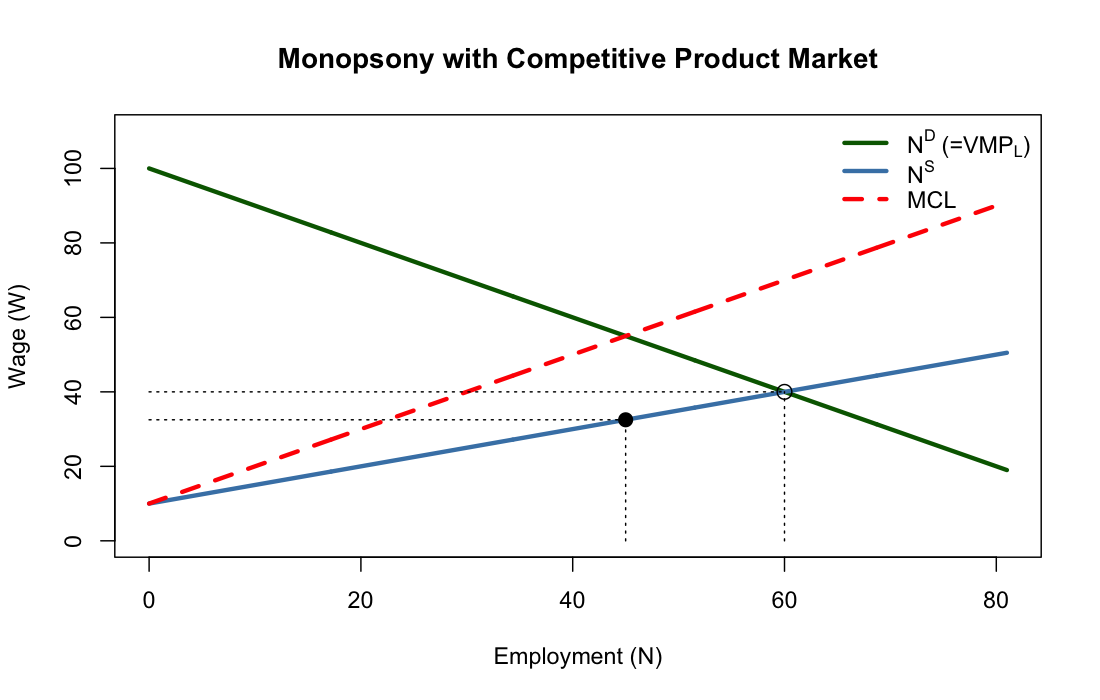
\includegraphics[width=1.1\linewidth]{F1}

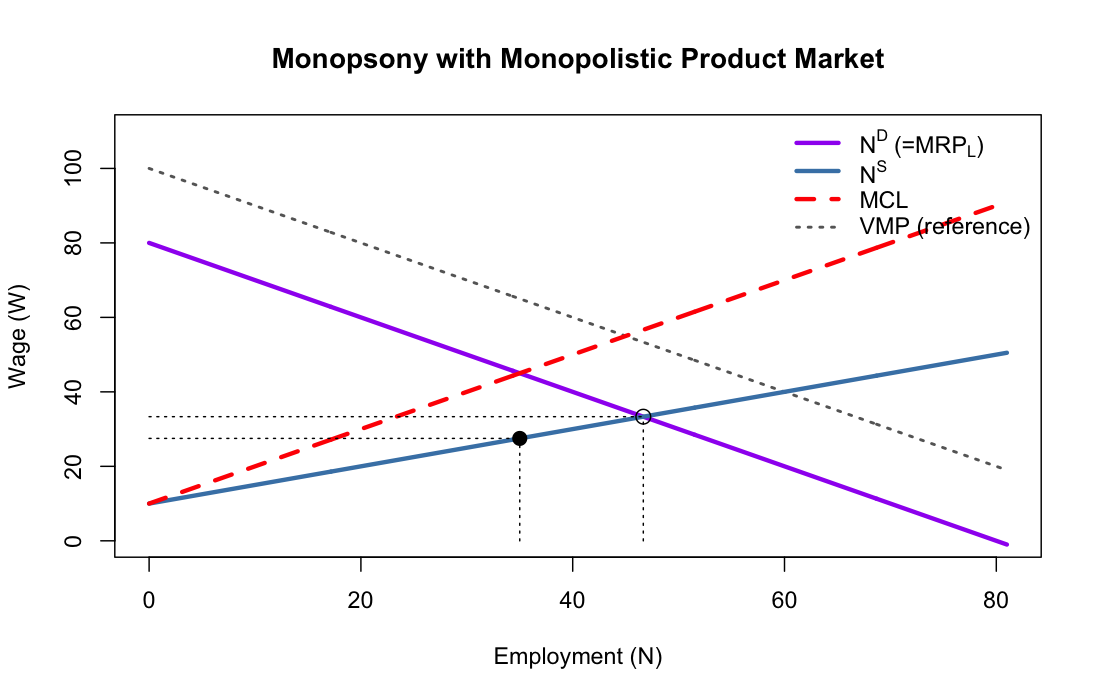
\includegraphics[width=1.1\linewidth]{F2}

\end{document}